\documentclass[a4paper,11pt]{article}
\usepackage{amsmath}
\usepackage{graphicx}
\usepackage{caption}
\usepackage{amssymb}
\usepackage{verbatim}
\usepackage{hyperref}
\usepackage{listings}
\usepackage{float}
\usepackage[thinc]{esdiff}
\usepackage{euscript}
\usepackage{subcaption}
\usepackage{enumitem}
\usepackage{commath}
\setlength{\parindent}{0em}
\newcommand*{\field}[1]{\mathbb{#1}}%
\usepackage{amsthm}
\newtheorem{claim}{Claim}
\captionsetup{labelformat=empty}
\usepackage[nottoc]{tocbibind}
\usepackage{adjustbox}
\DeclareMathOperator{\sech}{sech}


\begin{document}
\lstset{language = Matlab}
\begin{titlepage} % Suppresses displaying the page number on the title page and the subsequent page counts as page 1
	
	\center % Centre everything on the page
	
	\vspace*{3cm}

	\textsc{Mathematical Tripos, Part II}\\
	\textsc{Computational project}
	\begin{center}
      {\huge\bfseries Soliton Solutions of the KdV Equation\\[0.4cm]
}     \end{center}
	
	\vfill
	\vfill\vfill\vfill\vfill
	\includegraphics*[width = 2.675cm, height = 3.1cm]{coat.png}
	\vfill
    \textsc{University of Cambridge}
	
	\vspace*{\fill}
	\vfill
	{\large\today} 
	\vfill
	
\end{titlepage}
\setcounter{tocdepth}{3}
\tableofcontents
\newpage
\section{Question 1}
The KdV equation is 
\begin{equation}
u_t + uu_x + \delta^2u_{xxx} = 0.
\label{(1)}
\end{equation}
First we consider the general single-soliton solution $f(x-ct)$ into the KdV equation, we obtain the ODE: 
$$-cf'+ff'+\delta^2f''' = 0$$
Then we verify $f(x) = A{\sech}^2(\frac{x-x_0}{\Delta})$ satisfy the resultant ODE.
By direct substitution, writing $X = \frac{x-x_0}{\Delta}$, we have $$\frac{2c}{\Delta}{\sech}^2 X {\tanh} X -\frac{2A}{\Delta}{\sech}^4 X {\tanh}X +\frac{8\delta^2}{\Delta^3} (2\tanh X {\sech}^4 X-{\tanh}^3 X{\sech}^2 X)$$
By taking out the common factor$\frac{2}{\Delta}\sech^2 X \tanh X$, we obtain
$$ c-A\sech^2 X +\frac{4\delta^2}{\Delta^2} (2\sech^2 X - \tanh^2 X)$$
then by using $\Delta^2 = \frac{12\delta^2}{A}$, $c = \frac{A}{3}$ and $\sech^2 X + \tanh^2 X = 1$,  $$ =\frac{A}{3}(1+2\sech^2 X - \tanh^2 X-3\sech^2 X)  = 0$$
Therefore, the single soliton is indeed a solution of the KdV equation. \\
Now suppose we have cyclic boundary conditions 
\begin{equation}
u(x+1,t) = u(x,t). 
\label{(2)}
\end{equation}
\\We define $$M \equiv \int_{0}^{1} u(x,t) dx\ \ and\ \ E \equiv \int_{0}^{1} \frac{1}{2} u^2(x,t) dx. $$
Take the time derivative of M, we have:
$$\frac{dM}{dt} = \frac{d}{dt} \int_{0}^{1} u(x,t) dx= \int_{0}^{1} u_{t}(x,t) dx. $$ By the KdV equation \ref{(1)}, $$ = -\int_{0}^{1} uu_x + \delta^2u_{xxx} dx = -\left[\frac{u^2}{2}+\delta^2u_{xx}\right]_{0}^{1} $$
which is 0 by the cyclic boundary conditions \ref{(2)}. \\
Take the time derivative of E, we have:
$$\frac{dE}{dt} = \frac{d}{dt} \int_{0}^{1} \frac{1}{2}u^2(x,t) dx= \int_{0}^{1} uu_{t} dx. $$ By the KdV equation \ref{(1)}, $$ = -\int_{0}^{1} u^2 u_x + \delta^2uu_{xxx} dx = -\left[\frac{u^3}{3}-\delta^2uu_{xx}\right]_{0}^{1}+\delta^2\int_{0}^{1}u_xu_{xx}dx $$
$$= \left[\delta^2\left(uu_{xx}+\frac{u_x^2}{2}\right)-\frac{u^3}{3}\right]_{0}^{1}$$
which is 0 by the cyclic boundary conditions \ref{(2)}. 
Hence both M and E are first integrals of the KdV equation.
\section{Question 2}
By substituting the exact solution, we have the local truncation error:
\begin{align*}
e_{h,k} =& 2(u+2uu_x+\delta^2u_{xxx})+\frac{k^2}{3}u_{ttt}\\
&+\frac{h^2}{6}(3\delta^2u_{xxxxx}+2(u_{xxx}+u_{x}u_{xx}))+\mathcal{O}(k^4+h^4)\\
 =& \frac{k^2}{3}u_{ttt}+\frac{h^2}{6}(3\delta^2u_{xxxxx}+2(u_{xxx}+u_{x}u_{xx}))+\mathcal{O}(k^4+h^4) \\=& \mathcal{O}(k^2+h^2).
\end{align*}
So the numerical scheme has order $\mathcal{O}(k^2+h^2)$. \\
Rescale KdV equation with $t \rightarrow \tau t$, $x \rightarrow Lx$, we obtain:
$$\frac{u_t}{\tau} + \frac{uu_x}{L} + \frac{\delta^2}{L^3}u_{xxx} = 0.$$ Therefore, if we choose the scales $\tau = L = \delta$, we obtain the KdV equation with $\delta = 1$.\\
To ensure our numerical method converges for the rescaled equation,  we should alter our numerical scheme accordingly with $k \rightarrow \tau k$ and $h \rightarrow Lh$.
Since the stability condition for $\delta =  1$, the \textbf{rescaled} equation, is given by $$k \leqslant \frac{h^3}{4+h^2|u_{max}|},$$ we conclude that the stability condition for the original equation ($\delta \neq 1$) is $$(\delta)^{-1} k \leqslant \frac{{\delta}^{-3} h^3}{4+{\delta}^{-2} h^2|u_{max}|},$$ i.e. $$k \leqslant \frac{h^3}{4\delta^2+h^2|u_{max}|}.$$
The program can be found in \ref{P1}.\\
I used a explicit Euler scheme for the first step. It is easy to execute and not hard to obtain by adjusting the coefficients of the nonlinear and dispersive parts. \footnote{Alternatively, one could try a Crank-Nicolson for the first step. It is implicit, unconditionally stable and is second order in time, the same as the leap-frog method and hence the order of the whole method is preserved. But for such a scheme you will need to solve a nonlinear difference equation, which is hard. So here for simplicity reason I tried the explicit Euler, and it worked well.} The domain is chosen from -10 to 10, which is enough to show the soliton pattern. I chose $h = 0.05$ and $k = \frac{h^2}{4\delta^2+h^2A} = 0.0145$. The choice of k is to maintain stability, and the choice for h is such that the size of k is large enough to make sure of a manageable number of iterations to larger times. The amplitude of the exact solution is used in place of $|u_{max}|$. The numerical solution has two peaks. The propagation speed of the numerical solution is greater than that of the exact solution.
\begin{figure}[H]
 \center
 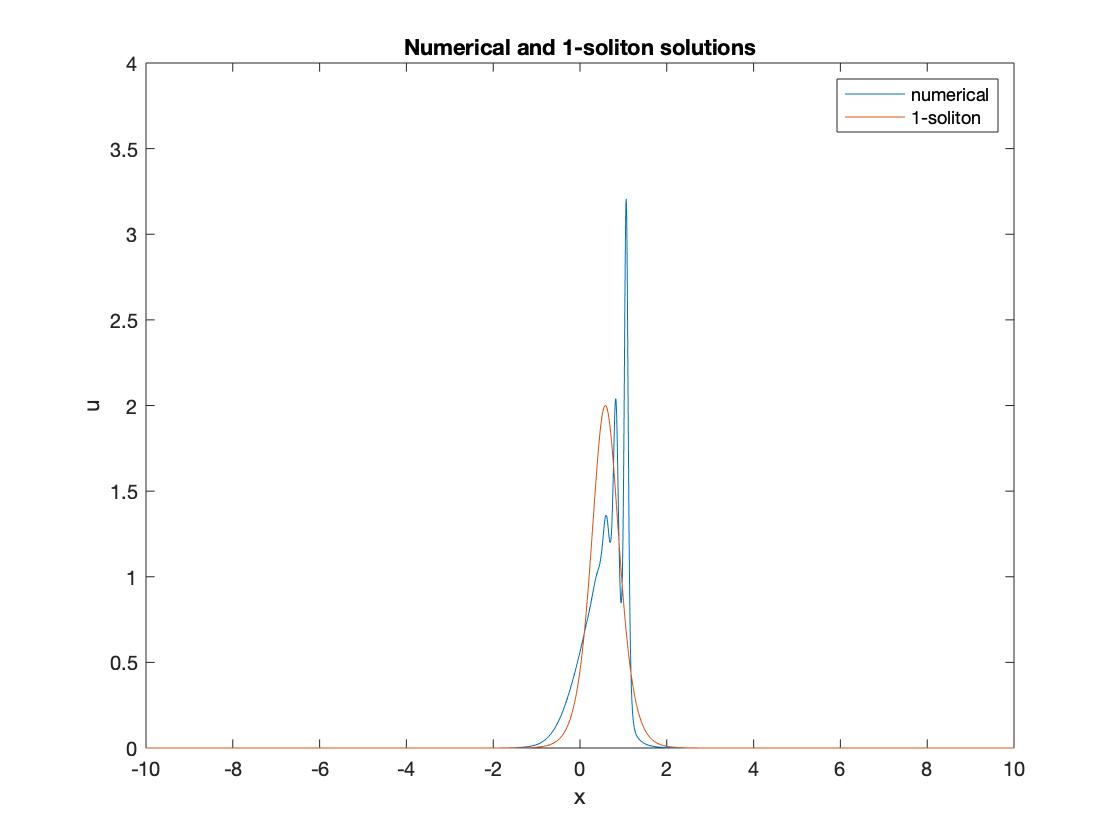
\includegraphics[width = 0.9\linewidth, height =8cm]{Q2.jpg}
 \caption{Figure 1.1: Numerical and 1-soliton solutions at t = 0.5}
\end{figure}
\newpage
\section{Question 3}
A right-propagating many-peak solution is to be expected. 
Evolution at representative times: 
\begin{figure}[H]
\begin{subfigure}{0.5\textwidth}
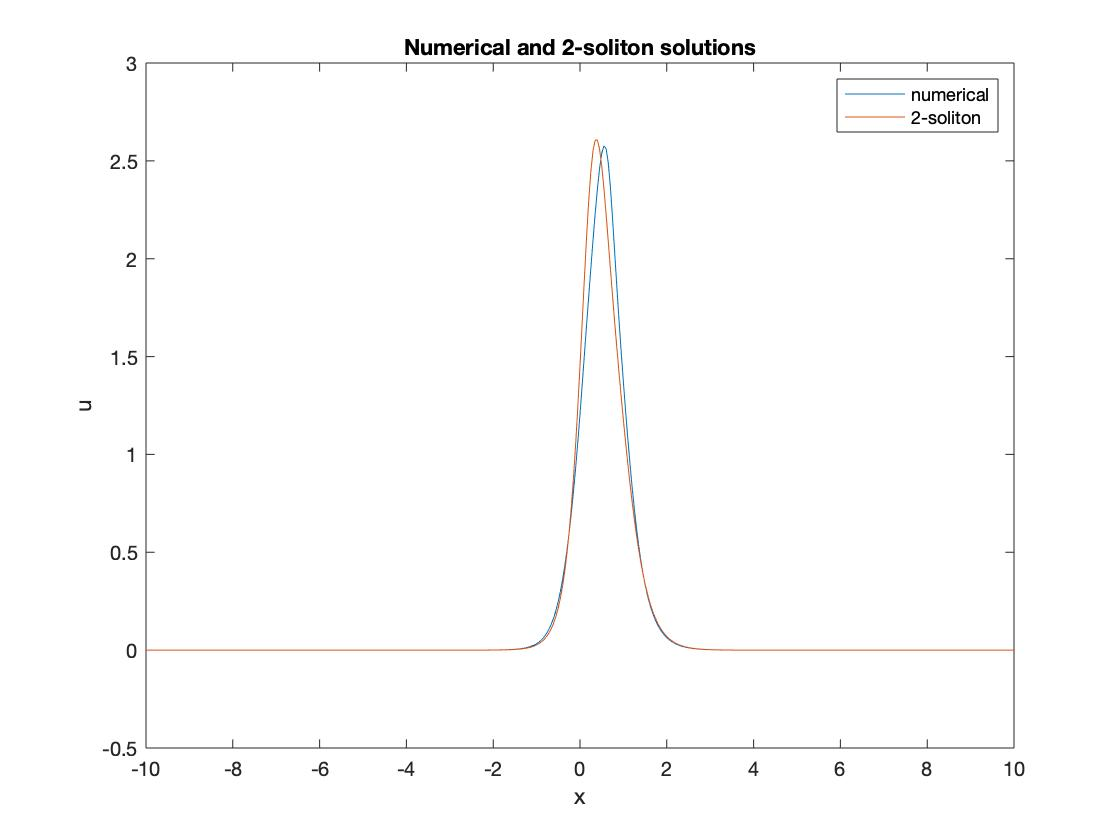
\includegraphics[width = \linewidth, height = 5cm]{Q3(1).jpg}
\caption{Figure 3.1: Numerical and 2-soliton solutions at t = 0.1}
\label{Q2(1)}
\end{subfigure}
\begin{subfigure}{0.5\textwidth}
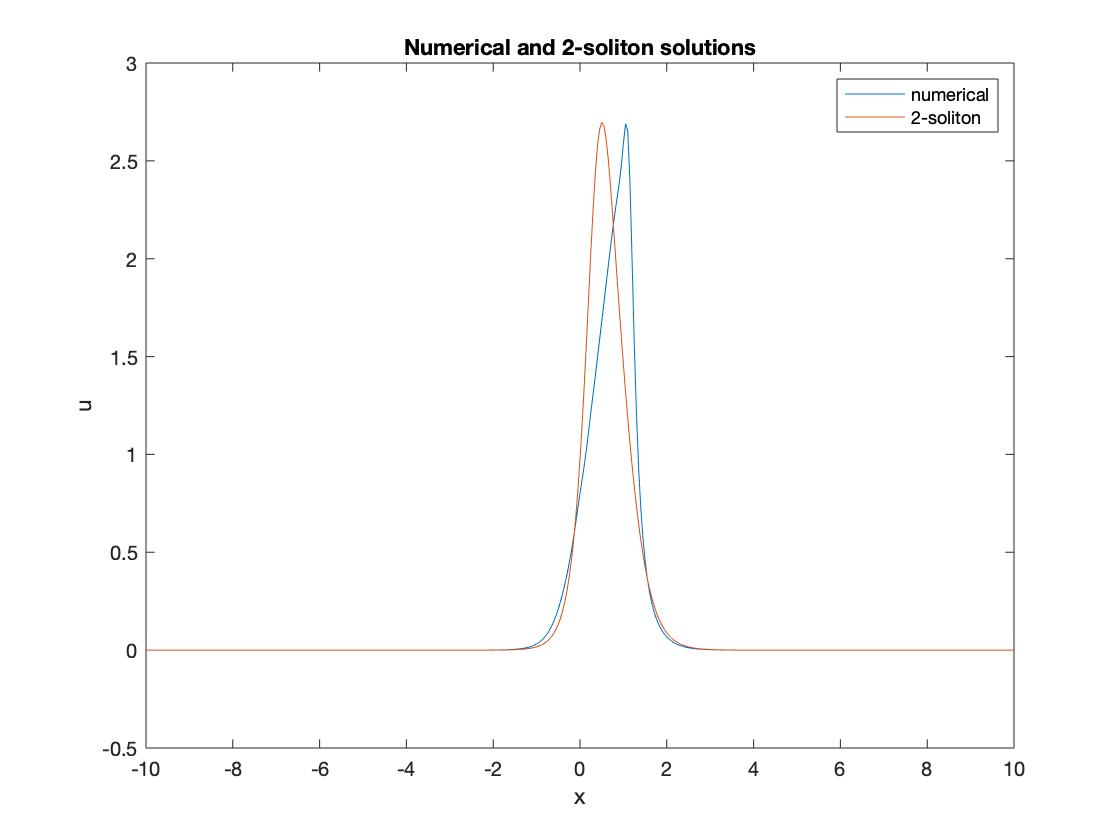
\includegraphics[width = \linewidth, height = 5cm]{Q3(2).jpg}
\caption{Figure 3.2: Numerical and 2-soliton solutions at t = 0.3}
\label{Q2(2)}
\end{subfigure}
\begin{subfigure}{0.5\textwidth}
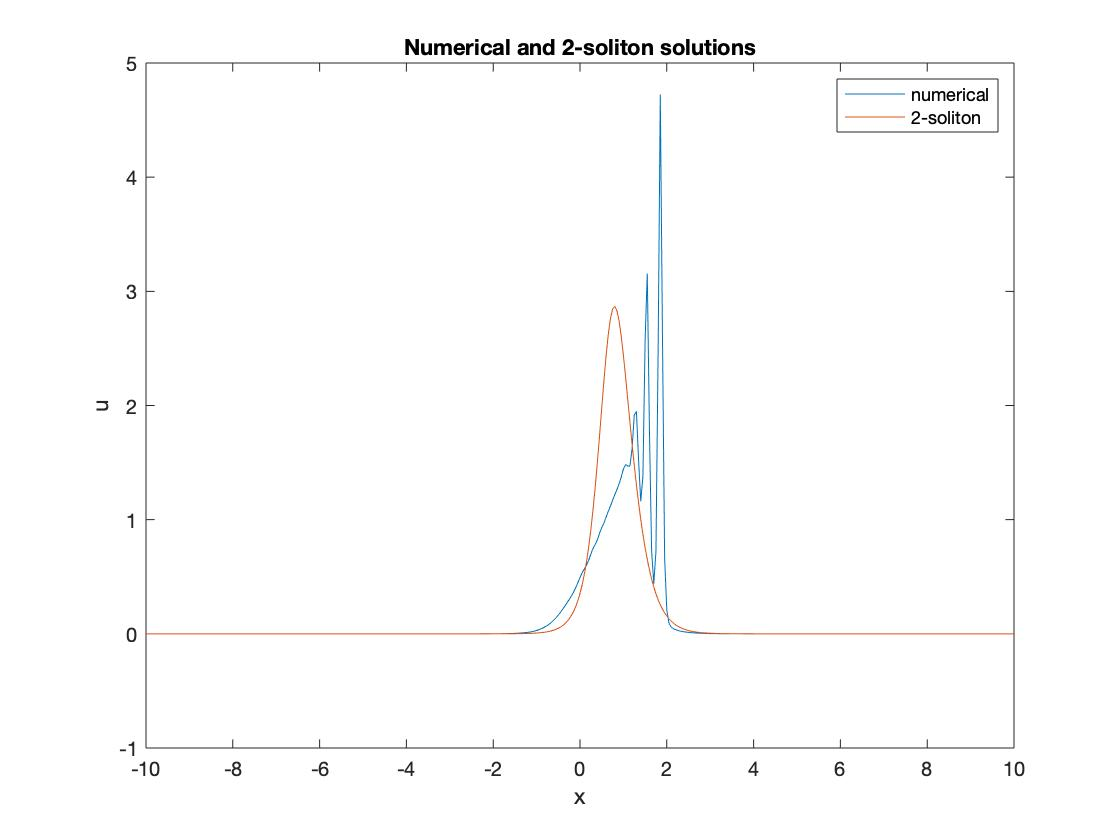
\includegraphics[width = \linewidth, height = 5cm]{Q3(3).jpg}
\caption{Figure 3.3: Numerical and 2-soliton solutions at t = 0.75}
\label{Q2(3)}
\end{subfigure}
\begin{subfigure}{0.5\textwidth}
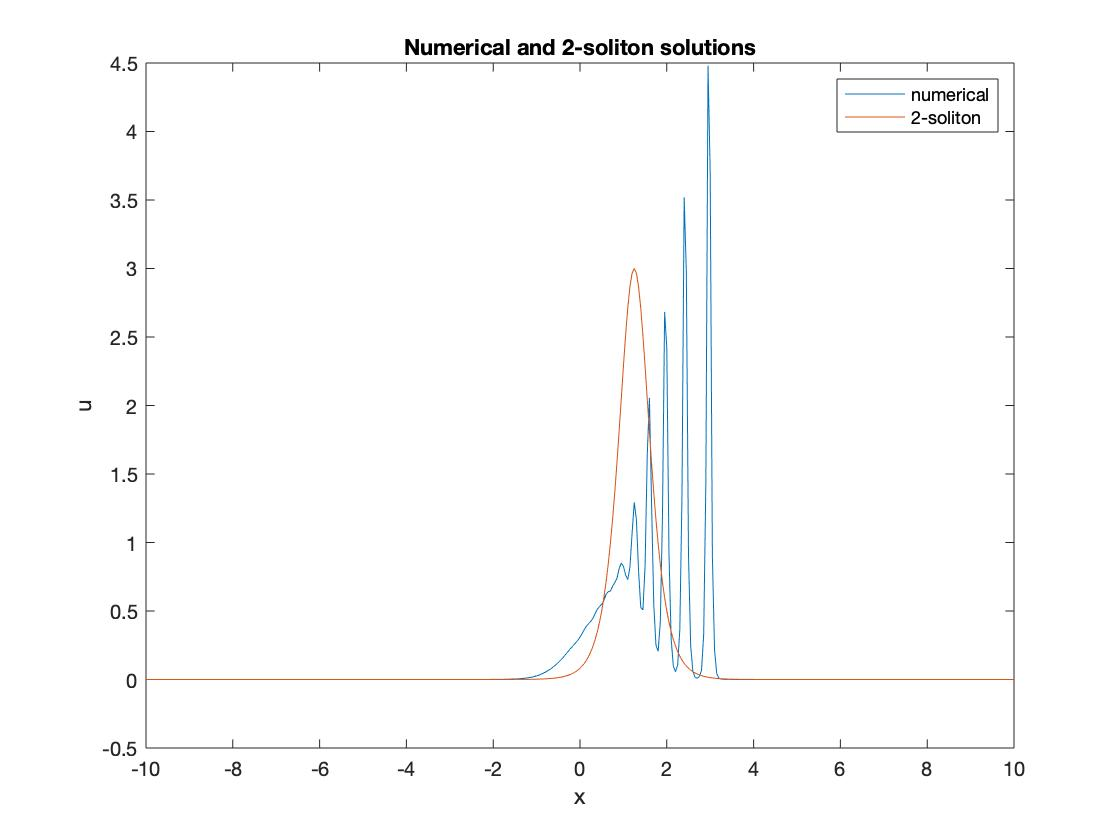
\includegraphics[width = \linewidth, height = 5cm]{Q3(4).jpg}
\caption{Figure 3.4: Numerical and 2-soliton solutions at t = 1.5 }
\label{Q2(4)}
\end{subfigure}
\begin{subfigure}{0.5\textwidth}
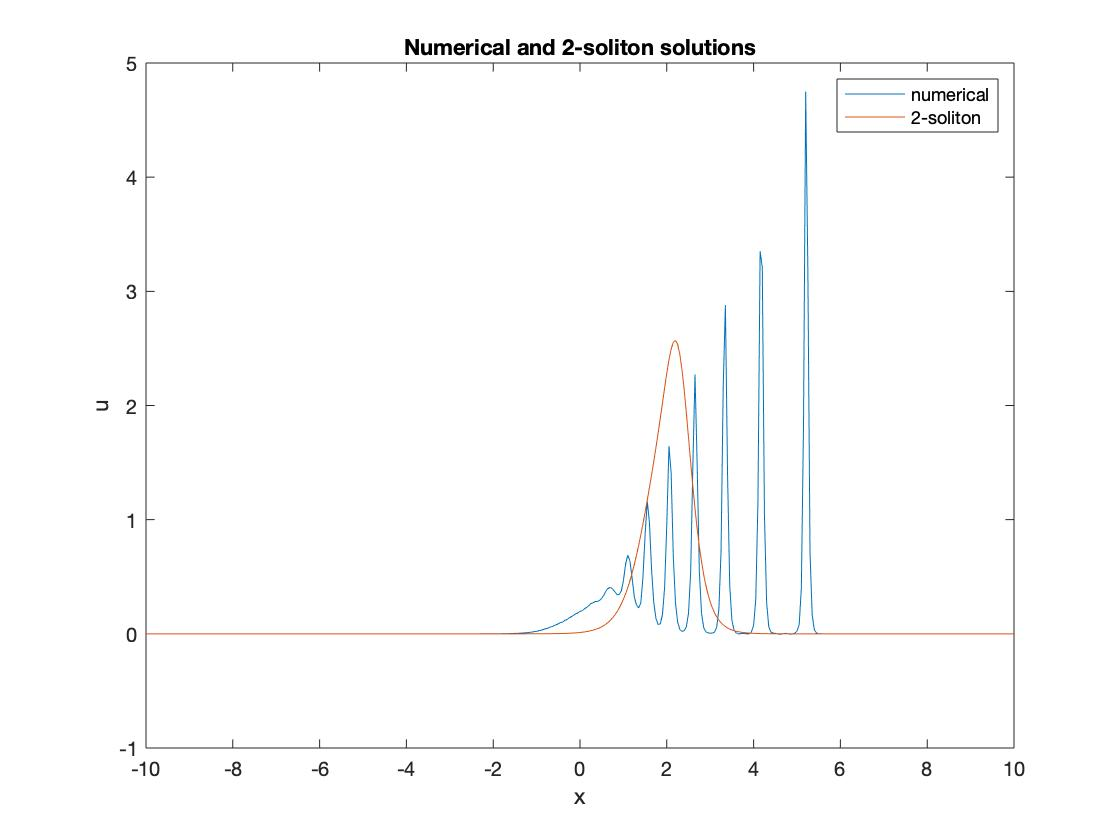
\includegraphics[width = \linewidth, height = 5cm]{Q3(5).jpg}
\caption{Figure 3.5: Numerical and 2-soliton solutions at t = 3}
\label{Q2(5)}
\end{subfigure}
\begin{subfigure}{0.5\textwidth}
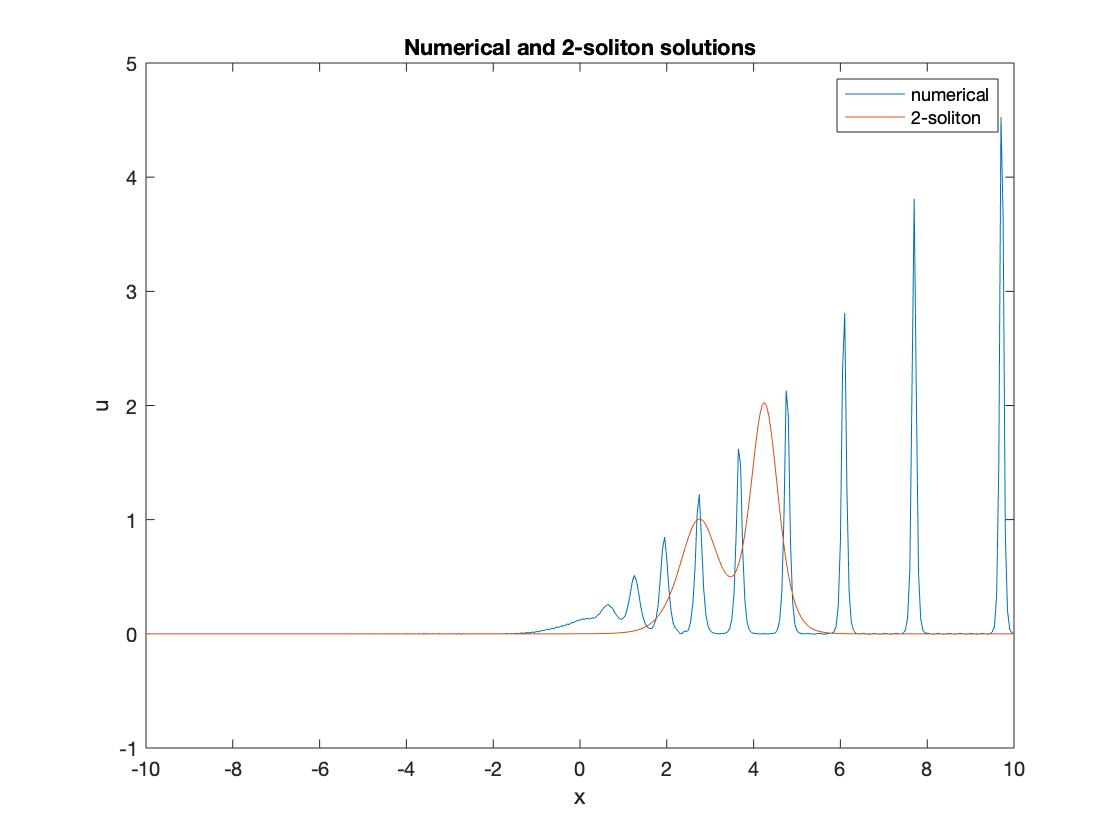
\includegraphics[width = \linewidth, height = 5cm]{Q3(6).jpg}
\caption{Figure 3.6: Numerical and 2-soliton solutions at t = 6}
\label{Q2(6)}
\end{subfigure}
\end{figure}
The following table\footnote{Values in the first column should all +k $\approx 3*10^{-5}$ (time-step)} shows the numerical 'mass' and 'energy' at these times, up to 4 significant figures. The variation of mass with time is small. And it can be observed that it is at least of $\mathcal{O}(10^5)$. The variation in energy is much larger, and from the 2-soliton case we can see that the energy is not conserved in time. Which means it is \textbf{not a solution} of the KdV equation. It also demonstrates the non-linearity of the Kdv equation as the superposition of two solutions is \textbf{not} another solution. 

\begin{table}[H]
\center
\begin{tabular}{|c||c|c|c|c||}
\hline 
(+k) & Numerical M & Numerical E&2-soliton M & 2-soliton E \\ 
\hline 
0.11452 & 57.9411 & 48.9154&57.9411 & 49.7327 \\ 
\hline 
0.3 & 57.9411 & 48.9145&57.9411 & 51.3766 \\ 
\hline 
0.75 & 57.9411 & 50.0413&57.9411 & 54.5506 \\ 
\hline 
1.5 & 57.9411 & 50.4534&57.9411 & 56.8920 \\ 
\hline 
3 & 57.9411 & 50.4967&57.9411 & 48.8834 \\ 
\hline 
\end{tabular} 
\end{table}

\section{Question 4}
If $\delta = 0$ we can use the method of characteristics to solve the problem. The characteristic is $x-ut$, hence $u(x,t) = f(x-ut)$. Therefore, the solution satisfies $u = \sin(2\pi x-ut)$. Since the gradient u is not monotonic in x, the characteristics cross and $|\frac{\partial u}{\partial x}|$ becomes unbounded. So we get shocks. By comparing the magnitudes of the nonlinear term $uu_{x}$ and the dispersive term $\delta^2 u_{xxx}$, we know that when $\frac{U^2}{L} \approx \frac{\delta^2 U}{L^3}$, i.e. $L \approx \frac{\delta}{U}$, the two terms balance. At first nonlinearity dominates and the peaks and troughs deepen. It will tend to forming a shock but before it occurs, the length scale will contract till it is small enough to balance the terms. After that the dispersion dominates and we are expected to get well-defined waves. The second peak emerges at $t \approx 0.09$, after that more peaks emerge and we should expect a train of waves with taller waves goes faster and shorter wave goes slower (which comes from the shallow water wave velocity$c^2 = g(h+a)$ where a is the amplitude of a soliton-like solution). The taller waves goes through the shorter waves and then reappear from the other end. 
\begin{figure}[H]
\begin{subfigure}{0.5\textwidth}
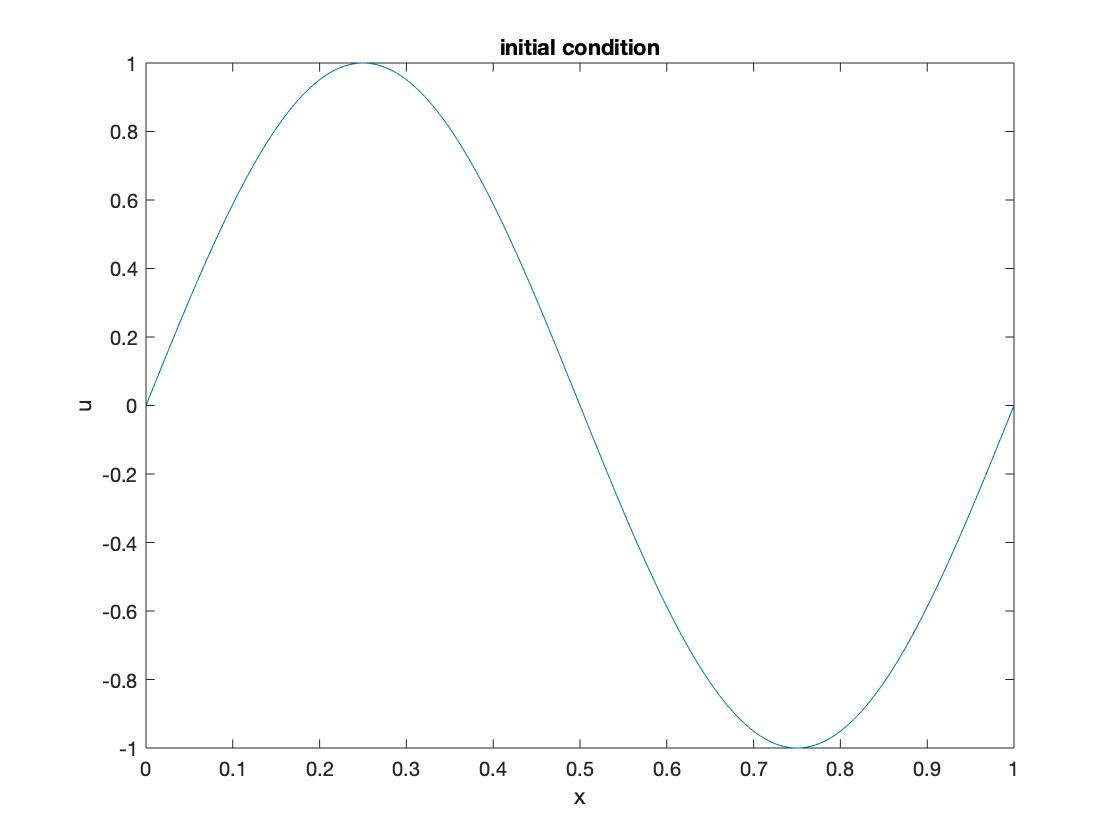
\includegraphics[width = \linewidth, height = 5cm]{Q4(6).jpg}
\caption{Figure 4.1: Initial condition}
\label{Q4(1)}
\end{subfigure}
\begin{subfigure}{0.5\textwidth}
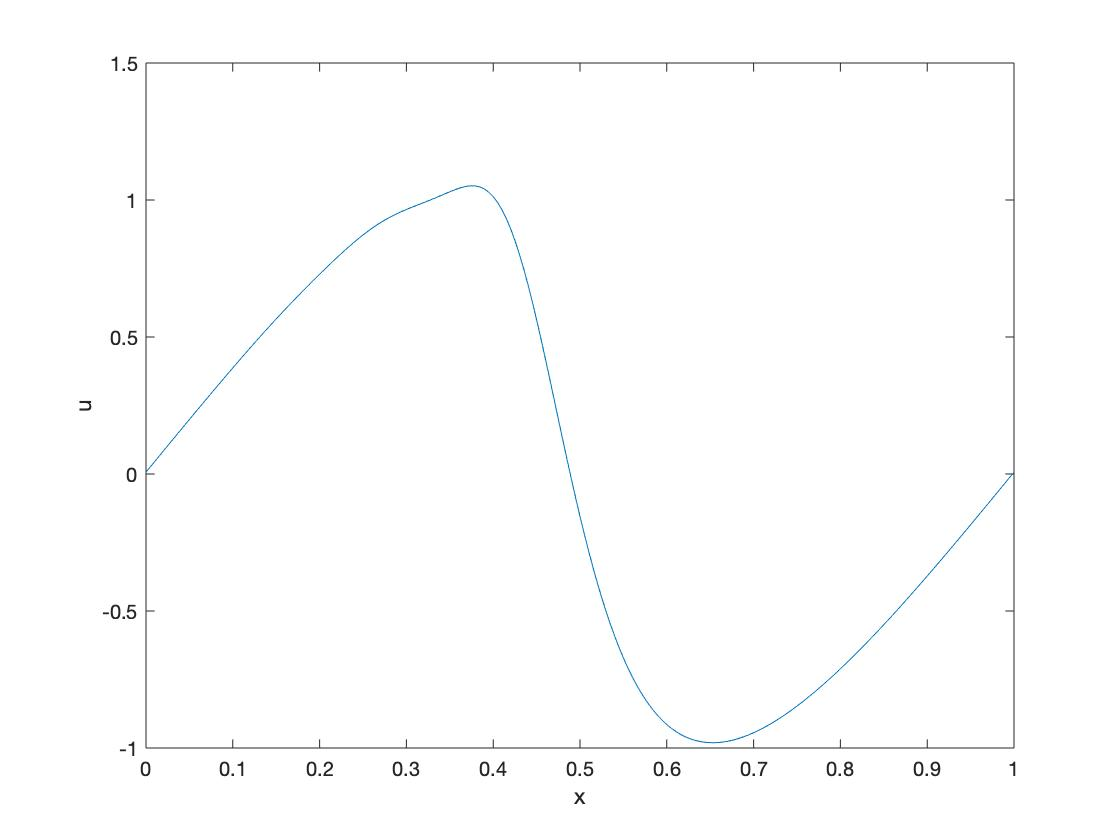
\includegraphics[width = \linewidth, height = 5cm]{Q4(5).jpg}
\caption{Figure 4.2: Numerical solution \\ at  t = 0.1}
\label{Q4(2)}
\end{subfigure}
\begin{subfigure}{0.5\textwidth}
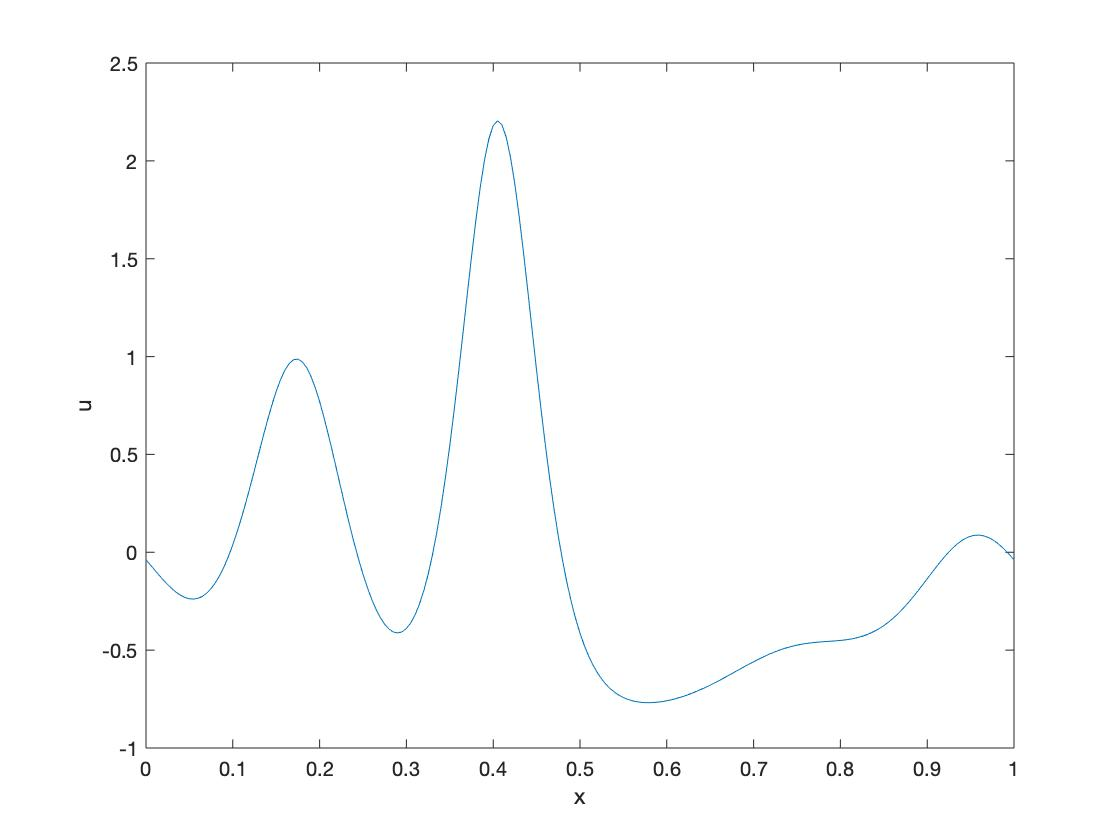
\includegraphics[width = \linewidth, height = 5cm]{Q4(4).jpg}
\caption{Figure 4.3: Numerical solution \\at t = 0.33}
\label{Q4(3)}
\end{subfigure}
\begin{subfigure}{0.5\textwidth}
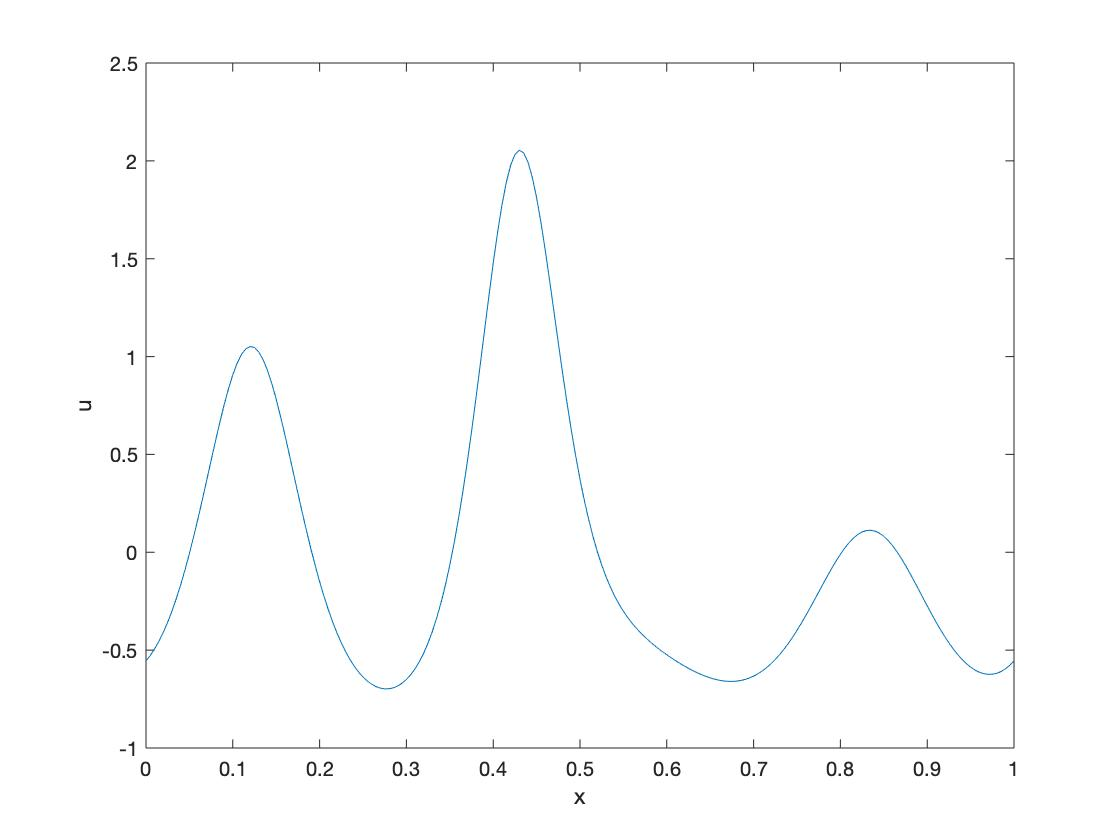
\includegraphics[width = \linewidth, height = 5cm]{Q4(3).jpg}
\caption{Figure 4.4: Numerical solution \\at t = 0.5}
\label{Q4(4)}
\end{subfigure}
\begin{subfigure}{0.5\textwidth}
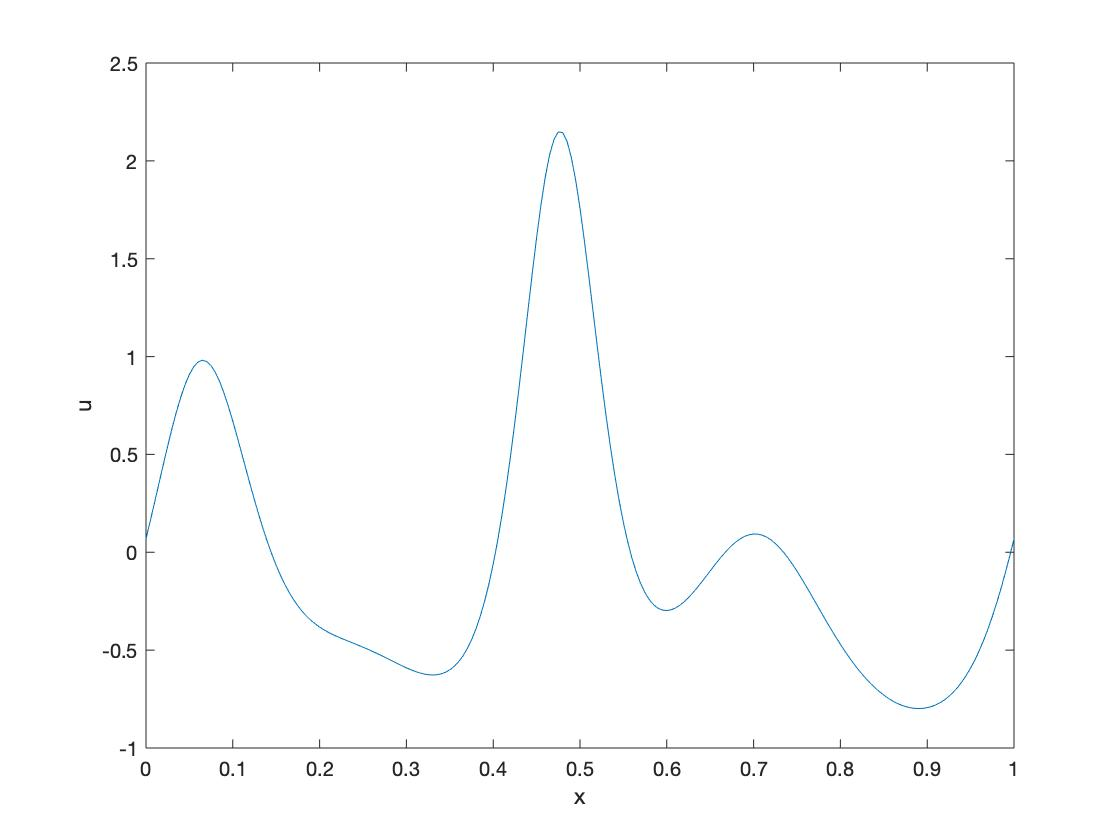
\includegraphics[width = \linewidth, height = 5cm]{Q4(2).jpg}
\caption{Figure 4.5: Numerical solution \\at t = 0.7}
\label{Q4(5)}
\end{subfigure}
\begin{subfigure}{0.5\textwidth}
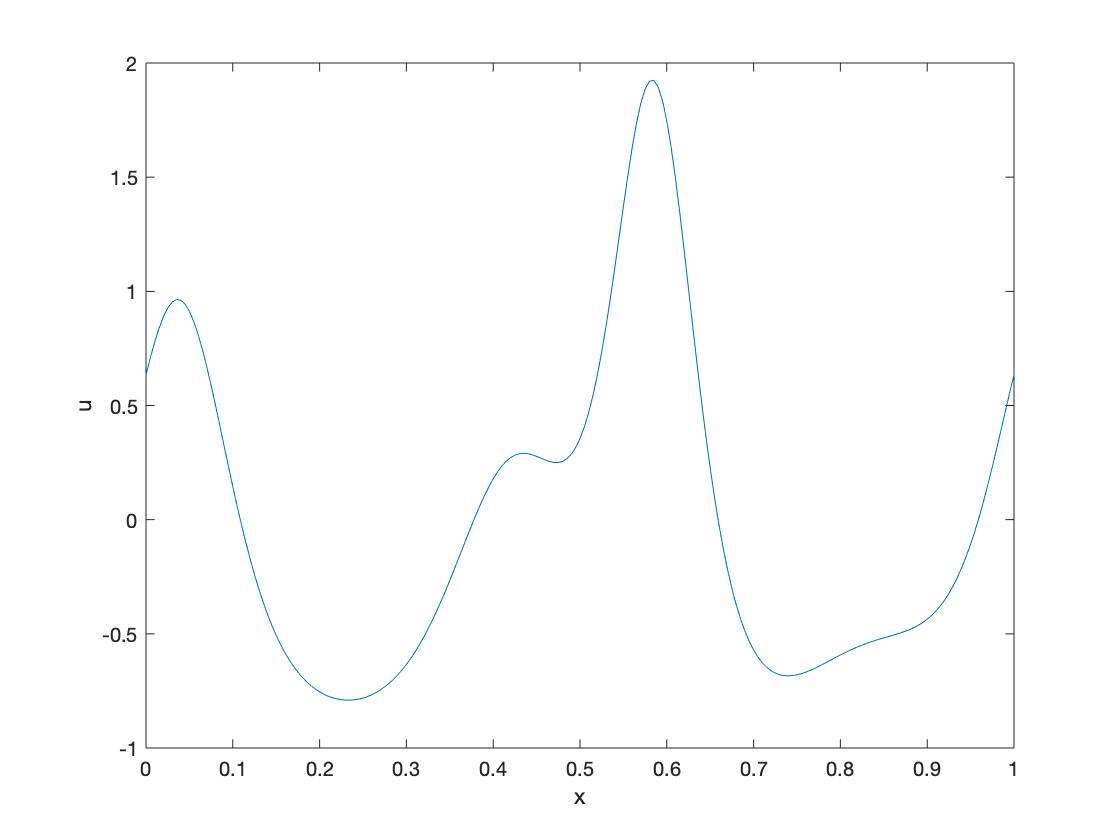
\includegraphics[width = \linewidth, height = 5cm]{Q4(1).jpg}
\caption{Figure 4.6: Numerical solution \\at t = 0.95 }
\label{Q4(6)}
\end{subfigure}
\end{figure}
From the numerical solution, the estimate is $t = 0.3327$ to 4 s.f.s as it is when steepening tops. \\
The time is earlier for large $\delta$ and later for smaller $\delta$, which is clearly because when $\delta$ is larger, the dispersion dominates quicker, and the balance between nonlinearity and dispersion is obtained sooner.

\begin{thebibliography}{9}
\bibitem{Drazin} 
Drazin, P.G. \& Johnson, R.S.
\textit{Solitons: An Introduction} 
CUP, 1989.
\end{thebibliography}
\newpage
\appendix
\section{Codes}
\subsection*{'1-soliton'}
\label{P1}
\lstinputlisting{Q2.m}
\subsection*{'2-soliton'}
\label{P2}
\lstinputlisting{Q3.m}
\subsection*{'last question'}
\label{P3}
\lstinputlisting{Q4.m}
\end{document}
\begin{thebibliography}{9}
\bibitem{Drazin} 
Drazin, P.G. & Johnson, R.S.
\textit{Solitons: An Introduction} 
CUP, 1989.
\end{thebibliography}